
% ====================================================================
\chapter{Sorted Sequences}

Jeden Tag produziert die Menschheit ungefähr 2,5 Trillionen Bytes Daten, das sind ungefähr 1,7 Megabyte pro Person und pro Sekunde.\cite{techjury:20} Diese unglaublich großen Datenmengen werden gespeichert, verändert, aufgerufen und wieder gelöscht. Dabei spielen ausgreifte Datenstrukturen eine entscheidende Rolle, damit schnell und flexibel Daten bearbeitet werden können. Bei der Entwicklung von Datenstrukturen erkannte man sehr zeitig, dass es einfacher ist, eine geordenete Ansammlung von Daten zu verwalten, als eine zufällige Anordnung derer. Lange bevor das Internet oder Computer überhaupt existierten, wandte man dies bei Wörterbüchern und Lexika an. Wenn wir etwas nachschlagen wollen, finden wir es dort viel schneller, weil wir uns sicher sein können, das "`foo"' nach "`bar"' im Wörterbuch stehen muss.
\par
Sortierte Sequenzen funktionieren nach dem gleichen Prinzip. Wie in \autoref{fig:NavStruct} zu sehen, besteht eine sortierte Sequenz aus zwei Teilen. Einer geordneten, doppelt verketteten Liste, in der die Elemente anhand ihrer Schlüssel sortiert sind. Das würde schon ausreichen, aber man verwendet zusätzlich noch eine Navigationsstruktur, welche das Auffinden von Elementen deutlich beschleunigt. In einer doppelt verketteten Liste würde das Lokalisieren von einem Element $e_n$ bis zu $n$ Schritte benötigen, also müssen im schlimmsten Fall alle Elemente der Liste durchlaufen werden, um das gesuchte Element zu finden. \footnote{Man schreibt auch: $\mathcal{O} (n)$} Im Gegensatz dazu hat eine sortierte Sequenz mit einem (a,b)-Baum als Navigationsstruktur (Vgl. \autoref{section:ab-trees}) drastisch verbesserte Laufzeiten von bis zu $\log n$. \footnote{$\mathcal{O} (\log n)$} \cite{Sanders:19}
\par
Vergleicht man sortierte Sequenzen mit anderen Datenstrukturen, kann man sowohl Nach- als auch Vorteile feststellen. Einerseits ist der Aufbau einer sortierten Sequenz komplizierter als der einfachererer Datenstrukturen wie Feldern, sie sind allerdings deutlich flexibler, da sie das Einfügen und Entfernen von Elementen effizient unterstützen. Im Vergleich zu Hashtabellen sind sie langsamer, aber mächtiger, da man auch Elemente findet, wenn man nach einem Schlüssel $s$ sucht, zu dem kein Element $e$ existiert (genauer: man findet das Element $e'$ für das gilt: $s'\leq s$).
\par
Somit können sortierte Sequenzen die Anforderungen Geschwindigkeit und Flexibilität sehr gut erfüllen. Auf der Grundlage des Buches \textit{"`Sequential and Parallel Algorithms and Data Structures - The Basic Toolbox"'} \cite{Sanders:19} werde ich die Funktionsweise von sortierten Sequenzen erklären, wie sie in Kapitel 7 des genannten Buches beschrieben werden. Das Hauptaugenmerk wird auf sortierten Sequenzen mit (a,b)-Bäumen als Navigationsstruktur liegen, es sind jedoch auch diverse andere Arten von sortierten Sequenzen vorstellbar, welche auch in logarithmischer Zeit arbeiten können.

\begin{figure}
    \begin{center}
        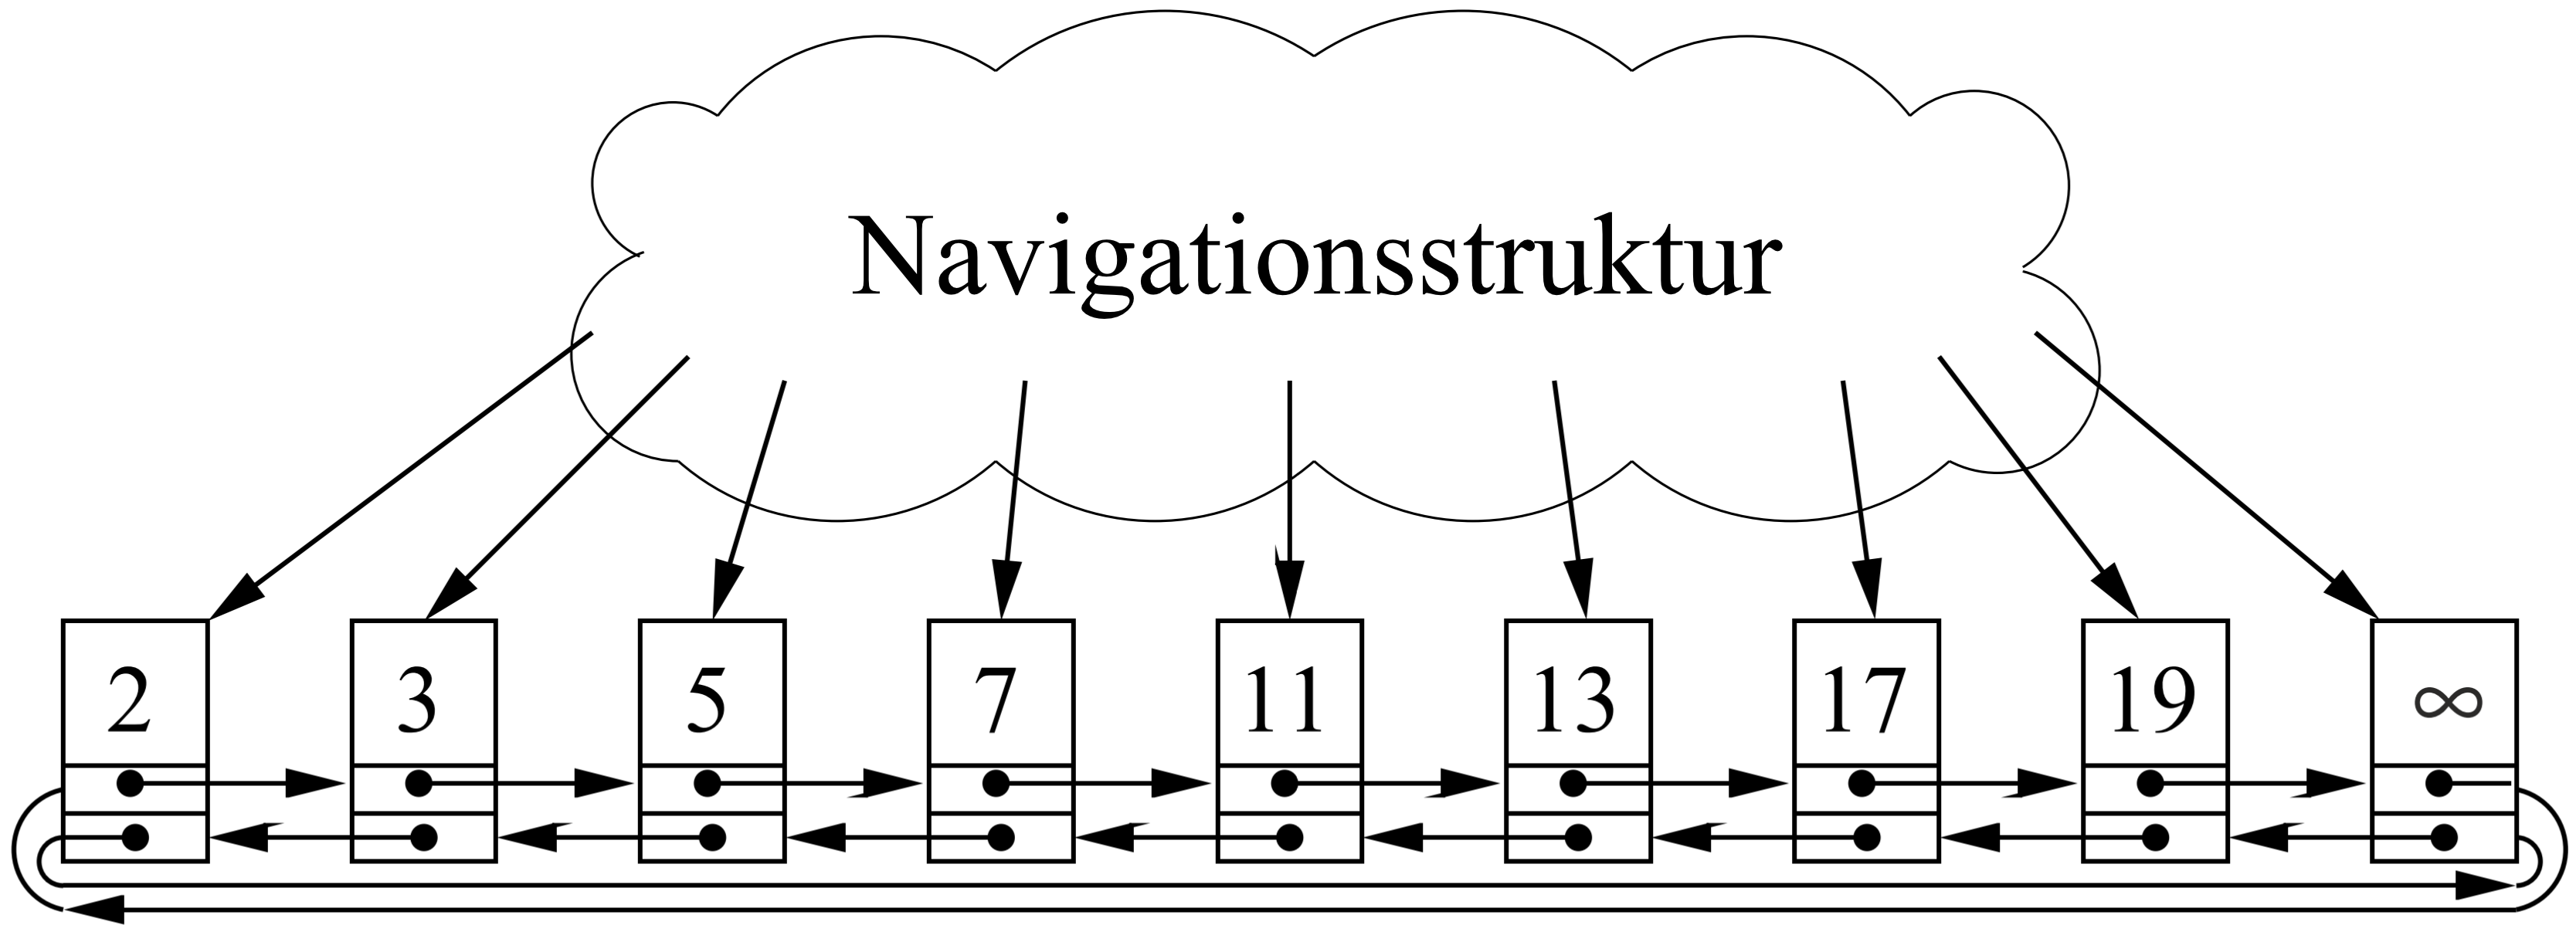
\includegraphics[width=0.8\linewidth]{assets/NavStruct.png}
        \caption{Eine sortierte Sequenz $\langle2, 3, \dots, 17, 19, \infty \rangle$, bestehend aus einer doppelt verketteten Liste und einer Navigationsstruktur. Das Dummy Element besitzt den Schlüssel $\infty$.\\\cite{Sanders:19}}
        \label{fig:NavStruct}
    \end{center}
\end{figure}


%--------------------------------------------------------------------
\section{Doppelt verkettete Listen}
\label{section:dll}

Verkettete Listen bestehen aus Elementen, die miteinander verknüpft werden. In einer einfach verketten Liste, zeigt jedes Element auf seinen Nachfolger, in einer doppelt verketteten Liste zeigt es zusätzlich auf seinen Vorgänger. Diese Struktur ermöglicht es, auf jedes Element zuzugreifen, auch wenn man anfangs nur ein Element gegeben hat. Des Weiteren sind vielseiteige Modifizierungen umsetzbar, namentlich das Einfügen und Löschen von Elementen oder von Teillisten, sowie das Verknüpfen von Listen. Ein Direktzugriff wird nicht unterstützt, da zuerst durch die Liste iteriert werden muss, um auf ein Element zuzugreifen.
\par
Einfach verlinkte Listen benötigen weniger Platz und sind schneller als doppelt verkettete Listen, weshalb es meistens besser ist, einfach verkettete Listen einzusetzen, wenn ihre Funktionalität ausreichend ist. Für sortierte Sequenzen benötigen wir jedoch doppelt verkettete Listen. \cite{Sanders:19}
\par
Die Anforderungen an eine doppelt verkettete Liste sind relativ simpel und führen bei Einhaltung zur korrekten Funktionsweise. Für jedes Element sollte $e_n$ gelten, dass der Vorgänger des Nachfolgers $e_{n+1}$ wieder das Element $e_n$ ist, und dass der Nachfolger des Vorgängers $e_{n-1}$ auch das Element $e_n$ ist. Somit können die Operationen $next$ und $previous$ ausgeführt werden, um durch eine doppelt verkettete Liste zu iterieren.\cite{Sanders:19}
\par
Doppelt verkettete Listen sind in sortierten Sequenzen für das Speichern der Daten zuständig, während die Navigationsdatenstruktur für das Lokalisieren derselben eingesetzt wird. In \autoref{fig:NavStruct} ist dies dargestellt. Zu beachten ist, dass das sogenannte "`Dummy Element"'\footnote{In \autoref{fig:NavStruct} besitzt es den Schlüssel $\infty$} kein Element im engen Sinne ist, da es ausschließlich die Pointer zu Nachfolger und Vorgänger enthält, jedoch keinen Wert. Dieses Dummy Element ist jedoch von entscheidender Bedeutung, da es so lange besteht, wie die Liste selbst besteht und somit immer den Zugriff auf alle restlichen Elemente gewährt. Diesen Weg habe ich auch in meiner Implementierung gewählt, worauf ich im Detail in \autoref{chapter:implementierung} eingehen werde.


%--------------------------------------------------------------------
\section{Binäre Suchbäume}
\label{section:binary-trees}

Eine sortierte Sequenz benötigt eine Navigationsstruktur, die das Auffinden von Elementen beschleunigt. Eine Möglichkeit kann sein, binäre Suchbäume zu benutzen. Dessen Funktionweise werden ich nun betrachten.
\par
Wer das Konzept der binäre Suche verstanden hat, kann dieses einfach auf binäre Suchbäume anwenden. Bei der binären Suche wird das "`Teile und Herrsche"'-Prinzip angewandt, man teilt den Datensatz, und vergleicht den Suchschlüssel mit der Stelle, an der man geteilt hat. Ist der Schlüssel kleiner oder gleich dem größten Element im linken Datensatz \footnote{bei Sortierung von klein nach groß, beziehungsweise von links nach rechts} wird die Suche auf den linken Datensatz beschränkt und wieder geteilt. Diese Vorgehensweise wird so oft wiederholt, bis nur noch ein Element übrig bleibt. Dieses Element muss dann den Schlüssel besitzen, wenn es im Datensatz vorhanden war.
\par
Ein binärer Suchbaum besteht aus "`Knotenpunkten"' und "`Blättern"'. Knoten speichern Schlüssel, welche den Weg zum gesuchten Element weisen. Diese Teiler-Schlüssel geben den maximalen Wert der Blätter in dem Unterbaum an, welcher sich auf der Linken Seite des Knotenpunktes befindet. Für alle Blätter im linken Unterbaum des Knotenpunktes mit dem Teilerschlüssel $s_t$ gilt $s \leq s_t$.
\par
Um ein Element mit dem Schlüssel $s$ zu finden, gilt also folgende Vorgehensweise: Man startet an der Wurzel des Baumes, sprich der Knotenpunkt ohne Eltern, der in einer visuellen Darstellung ganz oben stehen würde. Ist der Suchschlüssel $s_s$ kleiner oder gleich dem Teilerschlüssel $s_t$, steigt man in den linken Unterbaum ab. Ist $s_s>s_t$, führt man das Verfahren im rechten Unterbaum weiter. Falls das Element $e$ mit dem Schlüssel $s=s_s$ exisitiert,wird man es so finden. Falls das nicht der Fall sein sollte, gibt es zwei Möglichkeiten. Entweder der Unterbaum enthält den Vorgänger des Elementes gesuchten Elementes, $e'$ oder das gesuchte Element wäre der Nachfolger von $e'$. Ersteres tritt auf, wenn $s_s \leq Schlüssel(e')$ und zweiteres ist anzunehmen, wenn $s_s>Schlüssel(e')$. \cite{Sanders:19} Die doppelt verkettete Liste erledigt dann den Rest.
\par
Die Anzahl der Ebenen von der Wurzel bis zu den Blättern bezeichnet man als \textit{Höhe} des Suchbaumes. Bei Bäumen mit $n+1$ Blättern und einer Höhe von $\lceil \log (n+1) \rceil$ bezeichnet man als perfekt ausbalanciert.\footnote{$n$ Elmente und ein Dummy Element, daher $n+1$} Da an bei der Suche an jedem Knotenpunkt ein Schritt benötigt wird, entspricht die Zeit für das Suchen der Höhe des Baumes, das heißt $\mathcal{O}(\lceil \log (n+1) \rceil)$.\cite{Sanders:19} Dieser Wert ist sehr anstrebenswert, da er eine deutliche Verbesserung gegenüber anderen Datenstrukturen bietet, wie zum Beispiel die Doppelt verkettete Liste alleine. Wenn wir es mit einem gleichbleiben Datensatz zu tun hätten, wäre das ohne Abstriche zu genießen. Das entspricht aber leider nicht der Realität. Beim Einfügen und Entfernen von Elementen müsste der Baum balanciert bleiben, das Ausgleichen benötigt allerding viele Resourcen. Beim unkontrollierten Einfügen könnte es im schlimmsten Fall passieren, dass jeder Knotenpunkt auf der einen Seite zu einem Blatt zeigt und auf der anderen Seite zu dem restlichen Unterbaum. An diesem Punkt ist der Baum nicht besser als eine Liste.
\par
Da beim zufälligen Einfügen von Elementen nicht immer der schlimmste Fall eintritt, kann man davon ausgehen, dass die Höhe zu $\approx 2,99 \log n$ konvergiert. \cite{Sanders:19}


%--------------------------------------------------------------------
\section{(a,b)-Bäume}
\label{section:ab-trees}

Wie in \autoref{section:binary-trees} erwähnt, ist es sehr aufwendig, binäre Suchbäume zu balancieren. Bei jeder Operation \footnote{Einfügen und Entfernen von Elementen} müsste der Baum zu einem großen Grad umstrukturiert werden. An diesem Punkt setzen \textit{(a,b)-Bäume} an. Sie agieren nach dem gleichen Prinzip, besitzen eine Wurzel und Knotenpunkte, die zu den Blättern führen. Der Unterschied liegt in den Knotenpunkten. Anstatt von zwei Verzweigungen hat jeder Knotenpunkt zwischen $a \in \mathds{N}$ und $b \in \mathds{N}$ Unterbäume. Man bezeichnet die Anzahl der Unterbäume, die von einem Knotenpunkt ausgehen, als Grad $d$ des Knotenpunktes. Für (a,b)-Bäume gilt: $a \leq d \leq b$, wobei eine leere Sequenz eine Ausnahmen bilden kann, da diese nur aus der Wurzel mit einem Kind, dem Dummy-Element besteht.  Des Weiterein definiert man $a \geq 2$ und $b \geq 2 a - 1$, da somit $d$ flexibel genug ist, um sicherzustellen, dass alle Blätter die gleiche Tiefe haben. Die Wichtigkeit dieser Anforderung an $a$ und $b$ werden wir in \autoref{section:insert-remove} erkennen. In der Literatur \cite{Sanders:19} werde $a$ und $b$ meistens als $2$ und $4$ definiert, da diese Werte einfacher zu visualisieren sind und man somit das Konzept schneller versteht. In \autoref{fig:24Tree} ist ein solcher (2,4)-Baum dargestellt.
\par
Jeder Knotenpunkt besteht aus einem Feld von Zeigern zu den Unterbäumen (Blätter oder weitere Knotenpunkte) $c[1\dots d]$, einem Feld von Zeigern zu Teilerschlüsseln $s[1 \dots d-1]$ und dem Grad $d$, um zu uberprüfen, ob die Invariante $a \leq d \leq b$ erfüllt wird, oder ob Knotenpunkten geteilt oder zusammengeführt werden müssen.
\\
Man betrachte einen Knotenpunkt mit $s[1 \dots d-1]$ und $c[1 \dots d]$. Für alle Blätter mit Schlüssel $k$ am Fuße des Unterbaumes $c[i]$ gilt: $s[i-1] < k \leq s[i]$. Diese Invariante ermöglicht die Suche in (a,b)-Bäumen, welche in \autoref{section:locate} genauer betrachtet wird. Bei Betrachtung von \autoref{fig:24Tree}, erklärt sich auch, wieso nur $d-1$ Teilerschlüssel vorhanden sind, und nicht $d$. Alle Elemente, die einen Schlüssel haben, der größer als der Teilerschlüssel $s[d-1]$ ist, müssen zwangsläufig zu $c[d]$ gehören. Zur Vereinfachung definiert man $s[d]$ als $\infty$, da jeder verbleibende Schlüssel die Anforderung $k \leq \infty$ erfüllt. Mehr dazu in \autoref{chapter:implementierung}.
\par
Bevor in \autoref{chapter:operations} auf Operationen an sortierten Sequenzen mit (a,b)-Bäumen eingegangen wird, gilt es noch eine wichtige Beobachtung zu machen. Die Höhe eines (a,b)-Baumes beschreibt die Anzahl der Ebenen, beziehungsweise die maximale Anzahl von Knotenpunkten die man auf dem Weg von der Wurzel bis zu einem Blatt in einem gegebenen Baum maximal auffindet. Da man bei der Suche einen Baum von Wurzel bis zum gesuchten Blatt durchschreitet, ist die Höhe von entscheidender Bedeutung für die Laufzeit von Operationen. Für einen Baum mit $n$ Elementen beträgt die Höhe maximal $1+ \lfloor \log_{a}(n+1)/2 \rfloor$. \cite{Sanders:19}
\\
In diese Formel kann man beliebige Werte einsetzen und man merkt schnell, dass die Höhe bei steigender Anzahl von Elementen weiterhin klein bleibt. Diese Eigenschaft macht (a,b)-Bäume ideal für große Datenmengen, da schnelle Zugriffszeiten garantiert sind. In der vorliegenden Litartur liegt das Hauptaugenmerk auf (a,b)-Bäumen, und diesem Beispiel werde ich folgen.

\begin{figure}
    \begin{center}
        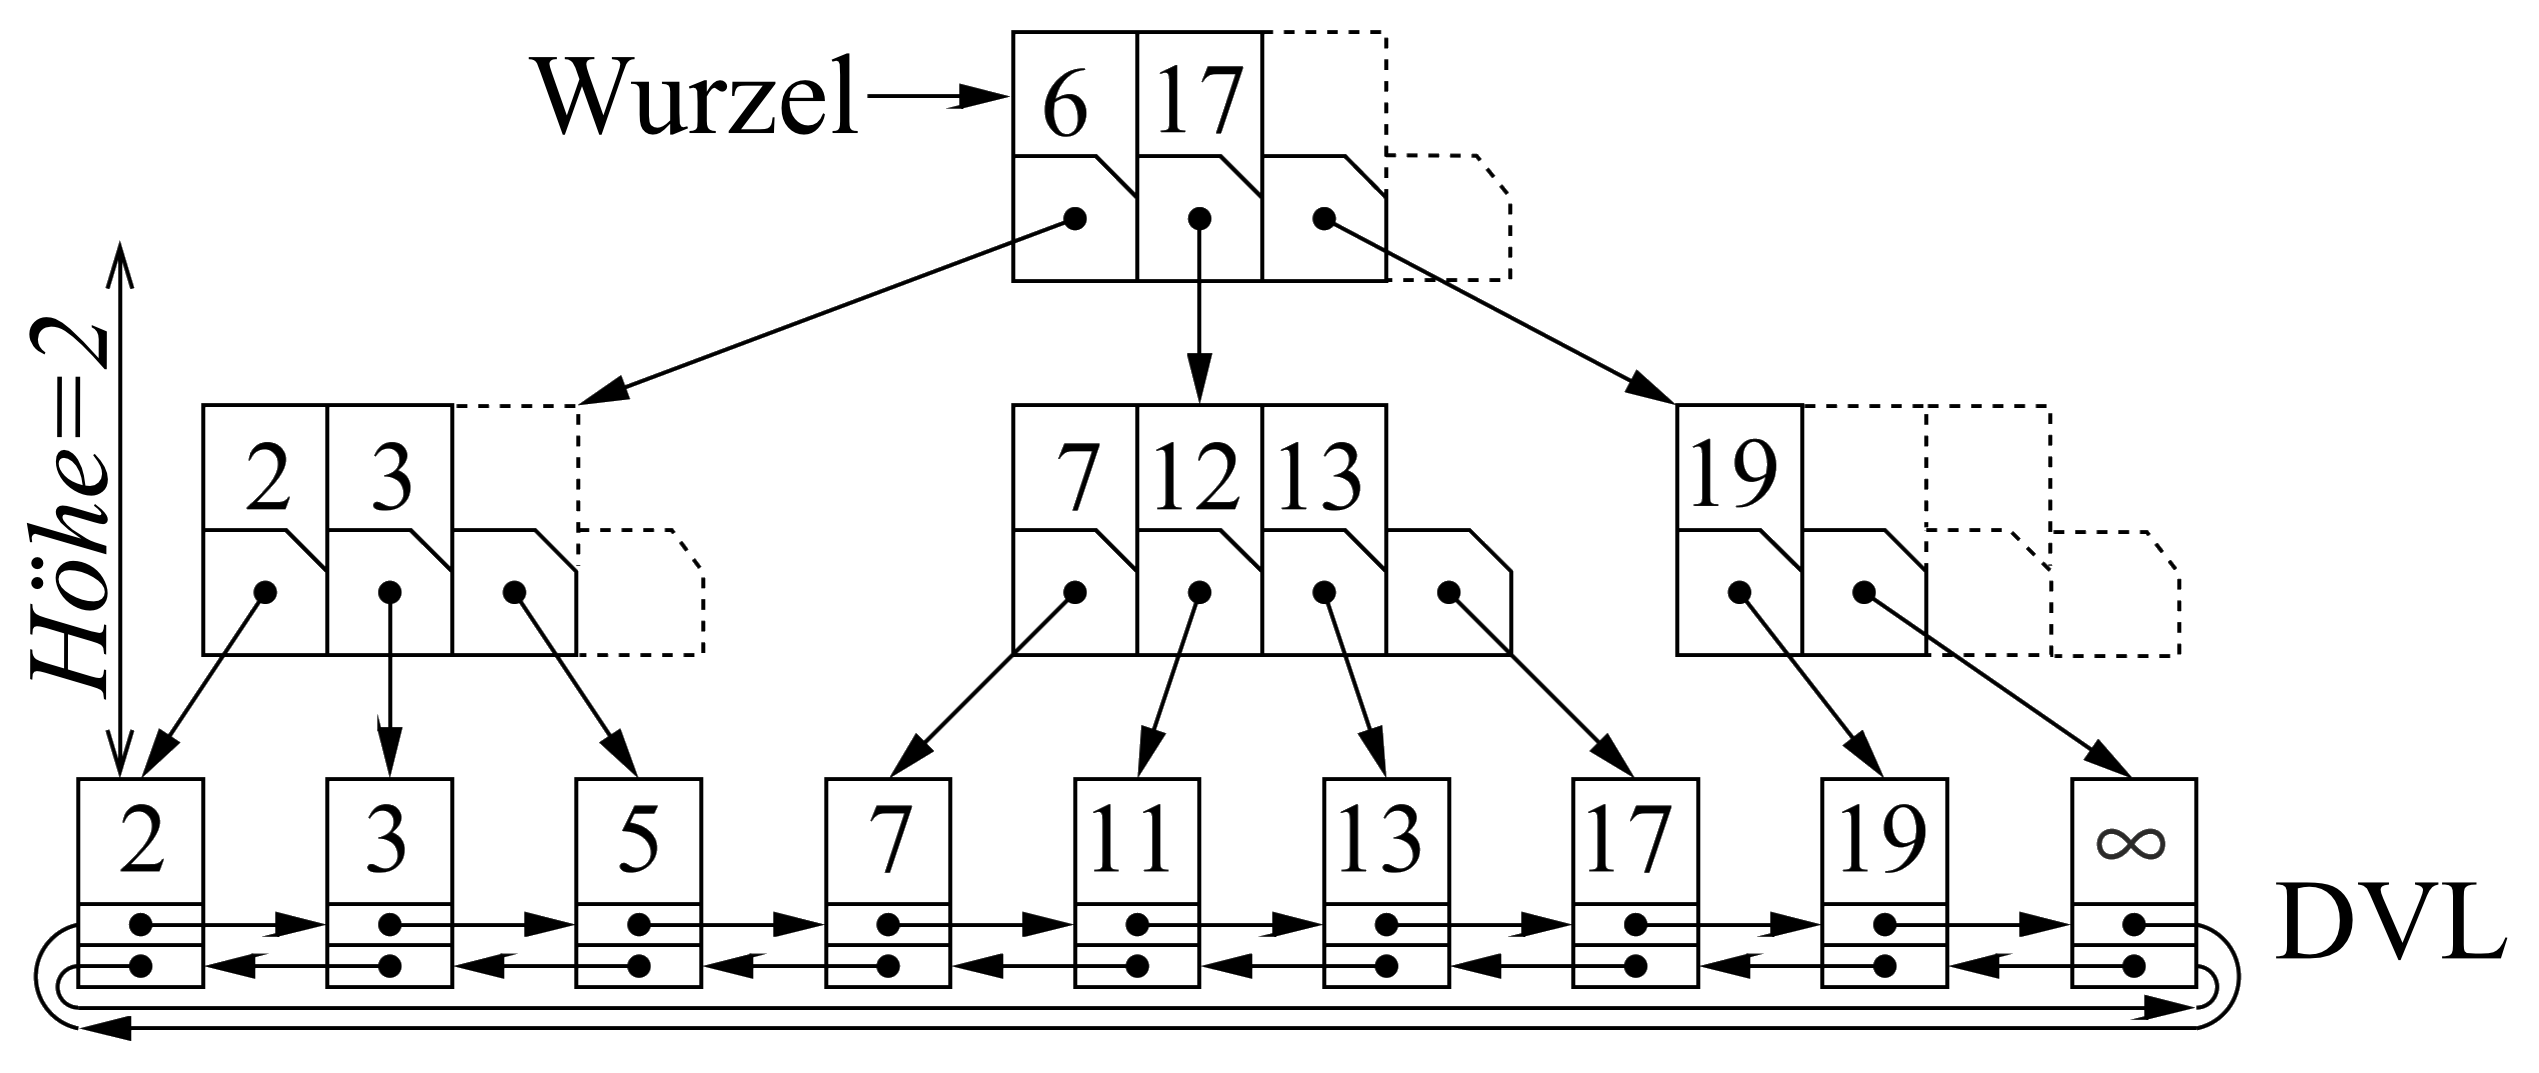
\includegraphics[width=0.7\linewidth]{assets/24tree.png}
        \caption{Ein (2,4)-Baum über einer doppelt verketteten List (DVL).\\\cite{Sanders:19}}
        \label{fig:24Tree}
    \end{center}
\end{figure}


% ====================================================================
\chapter{Operationen an Sortierten Sequenzen}
\label{chapter:operations}

In diesem Kapitel werde ich auf fünf verschiedene Operationen an sortierten Sequenzen eingehen. Ich werde auf das \texttt{Finden}, \texttt{Einfügen} und \texttt{Entfernen} von Elementen eingehen, sowie das \texttt{Teilen} und \texttt{Zusammenführen} von ganzen Sequenzen darstellen. Nach den einzelnen Erläuterungen werde ich des Weiteren auf die Laufzeiten dieser Operationen eingehen.
\par
Aufgrund der doppelt verketteten Liste sind weitere Operationen relativ einfach realisierbar, wie beispielsweise das finden des ersten und letzten Elementes in der Sequenz. Das Dummy Element besitzt Pointer zu Vorgänger und Nachfolger, also genau zum ersten und letzten Element. Deshalb können diese Operationen in konstanter Zeit durchgeführt werden.
\\
Außerdem sind Abfragen von Bereichen möglich, indem zuerst der Anfang durch \texttt{Finden} lokalisiert wird, und man dann Schritt für Schritt in der doppelt verketteten Liste voranschreitet, bis man auf ein Element trifft, welches größer als der gegebene Endpunkt ist.
\\
\cite{Sanders:19}

%--------------------------------------------------------------------
\section{Finden}
\label{section:locate}

Um ein Element zu finden, muss man dem richtigen Pfad folgen, der einem zum gewünschten Element führt. Der Schlüssel $s_s$ stellt die Eingabe dar. Wie bei binären Suchbäumen startet die Suche an der Wurzel, aber ist etwas komplizierter. Anstatt von nur einem Vergleich an jedem Knotenpunkt, müssen mehrere Vergleiche getätigt werden, da ein Knotenpunkt mehr als zwei Verzweigungen haben kann. An jedem Knotenpunkt soll, das Kind $c[i]$ identifiziert werden, für das gilt: $s[i-1] < k < s[i]$, wobei $s[i]$ den zu $c[i]$ zugehörigen Teilerschlüssel darstellt, $s[i-1]$ den Teilerschlüssel des Kindes links von $c[i]$ und $k$ den Suchschlüssel. In anderen Worten vergleicht man $k$ mit den Teilerschlüsseln, bis man den kleinsten Teilerschlüssel findet, der größer oder gleich $k$ ist. Aufgrund des in \autoref{section:ab-trees} beschriebenenen Aufbau kann man sich sicher sein, dass sich das gesuchte Element mit dem Schlüssel $k$ im Unterbaum des Kindes $c[i]$ befindet, insofern es existiert. Der Vorgang wird bei $c[i]$ weitergeführt, bis man den Fuß des Baumes erreicht.
\par
Um zu wissen, wann der Fuß des Baumes erreicht ist, übergibt man am Anfang der Suche den Parameter $h$, der die Höhe des Baumes angibt. Jedes Mal, wenn man eine Ebene weiter absteigt, reduziert man $h$ um $1$. Sobald $h = 1$ erreicht ist, weiß man, dass die Kinder des aktuellen Knotenpunktes Blätter sind, also Elemente enthalten.
\par
Falls das Element mit Schlüssel $k$ im Baum enthalten ist, endet die Suche bei diesem Element und ist erfolgreich. Ist dies nicht der Fall, enthält der aktuellen Knotenpunkt \footnote{Der letzte Knotenpunkt in der Suche, wenn $h = 1$} das Element mit $k'$, wobei $k' > k$ ist oder den Vorgänger dieses Elements bei $c[d]$. Dann gibt man das Nachfolger-Blatt von $c[i]$ zurück, welches einen größeren Schlüssel als $k$ haben wird.
\par
\textbf{Laufzeit: } Wenn man für die Vergleiche an den Knotenpunkten binäre Suche verwendet, braucht man maximal $\lceil \log b \rceil$ Vergleiche pr Knotenpunkt. Die maximale Anzahl an Vergleichen pro Suche ist $\lceil \log b \rceil (1+\log_a((n+1)/2))$, da der zweite Teil dieses Terms die Höhe des Baumes beschreibt, und somit auch die Anzahl an Knotenpunkten angibt, die von der Suche durchlaufen werden müssen. Da sich die Anzahl der Vergleiche auf einen konstanten Durchschnittswert belaufen \footnote{Da $b$ konstant ist und somit die Anzahl immer $\leq \log b$ ist}, ist die Laufzeit für das \texttt{Finden} eines Elementes linear von der Größe des Baumes und somit logarithmisch von der Anzahl $n$ der Elemente abhängig.\\
\cite{Sanders:19}

%--------------------------------------------------------------------
\section{Einfügen \& Entfernen}
\label{section:insert-remove}

Um eine Element einzufügen oder zu entfernen, muss zuerst sein Platz gefunden werden, beziehungsweise das Element selbst. Dies wird rekursiv durchgeführt, da es so möglich ist, den Pfad wieder zurückzuverfolgen, nachdem das Element eingefügt oder gelöscht wurde. Das Finden wird wie in \autoref{section:locate} beschrieben durchgeführt. Im Folgenden nennen wir das einzufügenende Element $e$ mit dem Schlüssel $k$. Durch die Suche erhalten wir das Element $e'$ mit $k'$. Wenn $k = k'$, können wir das Element ersetzen und die Operation ist abgeschlossen, da jeder Schlüssel maximal ein Mal in der sortierten Sequenz vorkommt. Wenn $k < k'$ ist, muss das neue Element $e$ vor $e'$ in der doppelt verketteten Liste eingefügt werden. Kommen wir zum letzten Fall, wenn $k > k'$ ist. In diesem Fall wird logischerweise $e$ nach $e'$ eingefügt. In den beiden letzten Fällen müssen die Zeiger der Nachbarn von $e$ angepasst werden.
\par
Nun folgt der komplizierte Part, die Knotenpunkte über $e$ müssen gemäß der Invariante $a \leq d \leq$ angepasst werden, falls sie nicht erfüllt ist. Beim Einfügen von Elementen kann es passierem dass der Grad $d > a$ wird, und wieder reduziert werden muss. Dazu wird der betroffene Knotenpunkt in der Mitte geteilt. Das wird erreicht, indem man auf der linken Seite des Knotenpunktes einen neuen Knotenpunkt erschafft und die linke Hälfte der Kinder $c$ mit den dazugehörigen Teilerschlüsseln $s$ zu diesem neuen Knotenpunkt verschiebt. Es ist darauf zu achten, die Werte von $d$ zu korrigieren und die Invariante $s[0] = - \infty, s[d] = \infty$ wiederherzustellen.
\\
Nun ist der Vorgang jedoch noch nicht abgeschlossen, da durch die Teilung der Grad der Eltern erhöht wurde. Da wir durch die Rekursion Zugriff auf die Elternknotenpunkte haben, können wir diesen Vorgehensweise so oft wiederholen, bis keine Teilung mehr nötig ist, oder wir bei der Wurzel angekommen haben, und diese notfalls auch geteilt haben. Beim Teilen der Wurzel muss eine neue Wurzel erstellt werden, und die Höhe des Baumes erhöht sich um eins.
\par
Beim Entfernen von Elementen kann es passieren, dass $d < a$ wird. Nun wird der betroffene Knotenpunkt $t$ mit seinem Nachbarn $u$ ausbalanciert. Es existieren zwei Fälle. Wenn $d$ von $u$ größer als $a$ ist, können eins oder mehrere Kinder von $u$ an $t$ übergeben. Wenn $d(u) = a$ ist, ist dies nicht möglich, da so $d(u) < a$ werden würde, und man das gleiche Problem wie anfangs hätte. Glücklicherweise kann man in diesem Fall $t$ und $u$ einfach miteinander kombinieren, und somit einen Knotenpunkt mit $d = 2a-1$ erschaffen. Dies kann die Invarianten des (a,b)-Baumes nicht verletzen, da die Anforderung $b \geq 2a-1$ existiert (Vgl. \autoref{section:ab-trees}).
\\
Wie beim Einfügen kann sich dieses Ausbalancieren bis zur Wurzel hocharbeiten und somit die Höhe des Baumes um eins verringern. Es gibt jedoch noch einen Sonderfall: Der Baum hatte bereits die Höhe 1, und besteht somit nur noch aus der Wurzel und dem Dummy Item. An diesem Punkt ist die Sequenz komplett geleert und die Höhe kann nicht weiter verringert werden.
\par
\textbf{Laufzeit: } Wie beim \texttt{Finden} sind die Laufzeiten von \texttt{Einfügen} und \texttt{Entfernen} linear abhängig von der Höhe des Baumes, und somit logarithmisch abhängig von der Anzahl der Elemente in der Sequenz.
\begin{quote}
    Für alle ganzen Zahlen $a$ und $b$ mit $a \geq 2$ und $b \geq 2 a - 1$, unterstützen (a,b)-Bäume die Operationen Einfügen, Löschen und Finden an sortierten Sequenzen der Größe $n$ in der Zeit $\mathcal{O}(\log n).$
        \hfill \cite{Sanders:19}
\end{quote}
Die hier beschriebene logarithmische Abhängigkeit der Laufzeiten von $n$ ist von entscheidender Bedeutung für sortierte Sequenzen und deren Erfolg. Sie erreichen damit sehr kleine Zugriffszeiten, die bei wachsender Länge $n$ der Sequenz immer weniger schnell ansteigen. Somit haben sortiere Sequenzen einen großen Vorteil gegenüber anderen Datenstrukturen, deren Zugriffszeiten bei wachsendem $n$ schneller ansteigen.

%--------------------------------------------------------------------
\section{Zusammenfügen \& Teilen}
\label{section:merge-split}

Das \texttt{Zusammenfügen} und \texttt{Teilen} von sortierten Sequenzen ist nicht nur praktsch im Umgang mit mehreren Sequenzen, sondern ist sogar essentiell für die Parallelisierung der bereits beschriebenen Operationen. Für das Zusammenfügen muss eine Anforderung erfüllt werden: Das größte Element von der ersten Sequenz $S_1$ darf nicht größer sein, als das kleinste Element der zweiten Sequenz, $S_2$. In anderen Worten dürfen sich die zwei Sequenzen nicht überlappen. Dies lässt sich schnell überprüfen, da das Dummy Element der doppelt verketteten Listen Zeiger auf das jeweils kleinste und größte Element enthält.
\par
Das Vorgehen beim Zusammenfügen ist wie folgt: Zuerst fügt man die beiden doppelt verketteten Listen zusammen, darauf achtend, das Dummy Element, welches sich in der Mitte der beiden Listen befinden würde, zu entfernen. Als nächstes wird die Wurzel des kleineren der beiden (a,b)-Bäume mit einem passenden Knotenpunkt zusammengefügt. Ein Knotepunkt gilt als passend, wenn bei ihm die Höhe des Baumes der Höhe des kleineren entspricht. Anders ausgedrückt: Wenn $Höhe(S_1) \geq Höhe(S_2)$ gilt, folgen wir von der Wurzel von $S_1$ dem Pfad, der am weitesten rechts ist $Höhe(S_1) - Höhe(S_2)$ Schritte. Nachdem wir so den richtigen Knotenpunkt gefunden haben, können wir ihn mit der Wurzel von $S_2$ zusammenfügen. Außerdem müssen die Teilerschlüssel angepasst werden. Ab diesem Punkt gleicht die Vorgehensweise dem Reparieren des Baumes wie beim Einfügen, da Knotenpunkte geteilt werden müssen und sich dies bis zur Wurzel fortsetzen kann.
\\
Wenn $Höhe(S_1) < Höhe(S_2)$ wahr ist, ist das Vorgehen analog, nur mit vertauschten Rollen. Außerdem muss man dem Pfad folgen, der ganz links ist - an dieser Seite fügt man $S_1$ an. \cite{Sanders:19}
\par
Werfen wir nun einen Blick auf das Teilen zweier Sequenzen. Das Ziel ist es, die Sequenz $S = \langle w, \dots , x,y, \dots, z \rangle$ in $S_1 = \langle w, \dots , x \rangle$ und $S_2 = \langle y, \dots , z \rangle$ zu teilen. Zuerst folgt man dem Pfad bis zum Blatt $y$ und teilt die doppelt verkettete Liste. Entlang dieses Pfades teilt man jeden Knotenpunkt in eine linke und rechte Hälfte. Jede Knotenpunkt-Hälfte bekommt dann die Kinder, die auf ihrer Seite des Pfades bis zu $y$ liegen. Durch dieses Vorgehen können nun Knotenpunkte entstehen, die einen Grad von Null bis $b$ haben. Jeder Knotenpunkt mit mindestens einem Kind, also $d = 1$, kann als Wurzel eines neuen (a,b)-Baumes betrachtet werden und mit der restlichen Baumhälfte zusammengefügt werden. Dies ist etwas einfacher als das Zusammenfügen zweier Bäume im allgemeinen Fall, da die doppelt verkettete Liste bereits zusammengefügt ist.
\par
\textbf{Laufzeit: } Die Laufzeit des Zusammenfügen von (a,b)-Bäumen hängt von der Differenz der Höhen von $S_1$ und $S_2$ ab, da für die Knotepunkte über der Stelle, wo man die Bäume zusammenfügt, eine Angleichung gemäß $a \leq d \leq b$ erfolgen kann. Wenn die Höhe der Bäume bekannt ist, entspricht die Laufzeit $\mathcal{O} (1 + | Höhe(S_1) - Höhe(S_2) |)$. Ist dies nicht der Fall, müssen die Höhe noch berechnet werden, und man erhält eine Laufzeit von $\mathcal{O} (max\{|S_1|, |S_2|\})$. \cite{Sanders:19}
\\
Beim Teilen beläuft sich die Laufzeit auf $\mathcal{O}(\log n)$. \cite{Sanders:19}


%====================================================================
\chapter{Parallelisierung}
\label{chapter:Parallelisierung}

Trotz der bereits schnellen Laufzeiten von Operationen wie \texttt{Einfügen} oder \texttt{Entfernen} bei sortierten Sequenzen mit (a,b)-Bäumen kann es von Vorteil sein, Parallelisierung einzusetzen. Es ist jedoch nicht einfach, sortierte Sequenzen so zu parallelisieren, dass mehrere Prozesse gleichzeitig auf den gleichen Baum zugreifen können und ihn verändern. Sowohl das Einfügen als auch das Entfernen von Elementen verändert die Struktur des Baumes \footnote{Mit Ausnahme der Fälle, dass beim Einfügen bereits ein Element mit dem Schlüssel exisitiert oder beim Entfernen der Schlüssel nicht vorhanden ist.}, sodass Probleme auftreten können. Es könnte beispielsweise passieren, das ein Prozess rekursiv im Baum absteigt, seine Operation ausführt, aber in dieser Zeit von einem anderen Prozess der Baum bereits verändert wurde. Dies führt unweigerlich zu Konflikten. Es benötigt großen Aufwand, diesen Problemen aus dem Weg zu gehen und es scheint sehr schwierig zu sein, signifikante Verbesserung der Laufzeit zu erreichen \cite{Sanders:19}
\par
Zur Parallelisierung von Programmen wird die Rechenlast auf mehrere Prozessoren, Threads oder auch virtualisierte Threads aufgeteilt. Somit kann ein großes Problem schneller bearbeitet werden, da es in kleinere Probleme aufgeteilt wird, welche schneller lösbar sind. Der Gesamtaufwand entspricht dann nur noch dem Aufwand, das Problem aufzuteilen, die kleinen Probleme gleichzeitig zu lösen, und dann die Lösungen zur Gesamtlösung zusammenzusetzen. Diese Herangehensweise bezeichnet man als das "`Teile-und-Herrsche"'-Prinzip.
\par
Betrachten wir zuerst das parallele Einfügen von mehreren Elementen. Zuerst teilt man die Sequenz mittels der in \autoref{section:merge-split} beschriebenen Operation Teilen so, dass man geeignete Bäume erhält, in die man die Elemente einfügen kann. Um die Elemente $\langle 3,5,7,11 \rangle$ in die sortierte Sequenz $S = \langle 1,2,6,10,12 \rangle$ einzfügen, würde man $S$ also erst in $S_1 = \langle 1,2,6 \rangle$ und $S_2 = \langle 10,12 \rangle$ aufteilen und dann parallel $\langle 3,5,7 \rangle$ in $S_1$ einfügen und $\langle 11 \rangle$ in $S_2$ einfügen. Danach können die Sequenzen $S_1$ und $S_2$ wieder zu $S = \langle 1,2,3,5,6,7,10,11,12 \rangle$ zusammengefügt werden. Dies ist nur ein Minimalbeispiel und kann so erweitert werden, dass große Felder von Elementen gleichzeitig eingefügt werden können. Besonders dann ergibt die Parallelisierung viel Sinn und resultiert in einer erkennbaren Verbesserung der Laufzeit. \cite{Sanders:19}
\par
Das "`Teile-und-Herrsche"'-Prinzip wird natürlich nicht nur bei sortierten Sequenzen angewandt, sondern findet auch in vielen anderen Algorithmen Anwendung. Ein prominentes Beispiel ist die binäre Suche, dort teilt man den Suchbereich immer wieder in kleinere Bereiche und vereinfacht so das Problem bis zum Trivialfall, wenn der Suchbereich nur einem Element entspricht und man es so entweder gefunden hat oder es nicht existiert.
\\
Bei der konkreten Umsetzung der Parallelisierung des Einfügen ist darauf zu achten, die sortierte Sequenz richtig zu teilen, und die richtigen Elemente an der richtigen Stelle einzufügen. Falls beim Zusammenfügen der resultierenden Sequenzen eine Überlappung auftritt, ist die Operation fehlgeschlagen und die Sequenzen sind nicht mehr zusammenführbar. Typische Fallstricke der Parallelen Programmierung, wie Wetlaufsituationen, bei denen zwei Prozesse auf das gleiche Objekt zugreifen oder Verklemmungen, bei denen die Prozesse auf einander warten \cite{Boles:08}, dürften nicht auftreten, da es sich bei den einzelnen Sequenzen um komplett selbstständige Objekte handelt.

%====================================================================
\chapter{Implementierung in Python}
\label{chapter:implementierung}

Die Implementierung von sortierten Sequenzen in einer Programmiersprache erwies sich für mich als Berg- und Talfahrt. Zuerst begann ich, doppelt verkettete Listen in \textit{C} zu programmieren, was auch innerhalb eines Nachmittages Erfolg hatte. Danach versuchte ich mich an (a,b)-Bäumen, musste jedoch schnell feststellen, dass ich an meine Grenzen stieß, was C-Programmierung angeht. Ich hatte erst dieses Semester angefangen, C zu lernen, und kam noch nicht mit Speicherverwaltung und Datentypen zurecht.
\\
Also entschloss ich mich, die Entwicklung auf Python zu verlegen, und fing wieder mit doppelt verketteten Listen an. Im Nachhinhein denke ich, das dies die richtige Entscheidung war, denn in Python konnte ich echt objektorientiert programmieren, was in C nur behelfsmäßig mit Hilfe von \texttt{structs} möglich war. Außerdem besitze ich in Python etwas mehr Erfahrung, ein gutes halbes Jahr.
\par
Unter \url{https://github.com/joshuajeschek/SortedSequences} ist der Code meine Implementierung einsehbar. Alle dort verfügbaren Dateien sind mit Kommentaren zu den Klassen und Methden versehen, deshalb werde ich nicht auf jede einzelne Methode eingehen. Für meine Implementierung habe ich insgesamt 4 Klassen benutzt. \texttt{Leaf} und \texttt{DoublyLinkedList} für doppelt verkettete Listen (siehe \textit{dll.py}), sowie \texttt{Node} und \texttt{ABTree} für (a,b)-Bäume(siehe \textit{abTree.py}). Im Folgenden werde ich die zugehörigen Methoden erläutern, und Anmerkungen zu meiner Implementierung machen.
\par
Das Programmieren von doppelt verketteten Listen war recht unkompliziert. Methoden wie \texttt{locate} basieren auf den Referenzen zu den Vor- und Nachfolgern der einzelnen Elemente. Dies war jedoch nur die Vorbereitungsarbeit für sortierte Sequenzen mit (a,b)-Bäumen. Die Klassen \texttt{Node} und \texttt{ABTree} waren durchaus komplizierter.
\\
Ich orientierte mich am Pseudocode aus dem Buch (\cite{Sanders:19}), was jedoch nicht immer ohne Probleme "`übersetzbar"' war. Der Pseudocode ist an C++ angelegt. Manche Vorgänge konnte ich durch die Benutzung von Python vereinfachen, manche stellten sich als etwas schwieriger heraus. Im Pseudocode findet man oft Notationen, um auf die Elemente eines Arrays zuzugreifen, wie beispielsweise \texttt{s'[b+2-d..b]}. Hier ist die obere Grenze als inklusiv aufzufassen. In Python müsste man also schreiben \texttt{s'[b+2-d : b+1]}, da dort die obere Grenze exklusiv ist.
\\
Da es sich beim Umsetzen der Methoden in Python nicht nur um ein stures Abschreiben handelte, konnte ich so die Funktionsweise komplett verstehen, was alleine durch das Lesen des Buches nicht der Fall war. Nach der Behebung von mehreren Fehlern die sich eingeschlichen hatten, wusste ich genau, worauf bei Operationen \texttt{locate}, \texttt{insert}, \texttt{remove} zu achten ist. Dies half mir dann auch, \texttt{merge} umzusetzen, wo es nur die Beschreibung im Text als Anhaltspunkt gab. Die Funktion \texttt{mergeRec} hätte man vielleicht etwas kürzer gestalten können, wenn man sie in zwei Funktionen aufteilt. Eine für den Fall, dass der Baum von Sequenz 1 höher als der von Sequenz 2, und eine für die restlichen Fälle. Ich habe jedoch eine Funktion für beide Fälle definiert, bei der man mittels der Variable \texttt{l\_r} angibt, ob man auf der rechten oder linken Seite des Baumes absteigt. Bei der Übergabe von $\infty$ steigt man auf der rechten Seite ab, bei der Übergabe von $-\infty$ auf der linken Seite. Das ermöglichen die Teilerschlüssel \texttt{self.s[0]} und \texttt{self.s[d]}, welche bei jedem Knotenpunkt den Weg nach links und rechts weisen.
\par
Es gibt allerdings auch eine offensichtliche Schwäche in meiner Implementierung, in der Methode \texttt{locateLocally} der Klasse \texttt{Node}. Die Suche nach dem passenden Teilerschlüssel in \texttt{self.s} erfolgt dort mittels einer einfachen Schleife, die den ersten Index des ersten Wertes zurückgibt, für den gilt \texttt{$key \leq self.s[i]$}. Hierbei handelt es sich um eine einfache Lösung, denn wir wollen den kleinsten Index erhalten, für den dies gilt. Eine potentiell schnellere Lösung würde den Einsatz von binärer Suche beinhalten, was aber durch den Fakt erschwert werden würde, dass man ein Ergebnis erhalten kann, welches nicht der kleinste Index ist, für den die Bedingung gilt. Deshalb müsste man dies dann nochmals dann nochmals überprüfen. Bei kleinen Werten für $b$ ist die Auswirkung nicht bemerkbar, die Ausführung kann sogar etwas schneller als mit binärer Suche sein, wenn sich der Wert am Anfang von \texttt{self.s} befindet. Außerdem spart man Zeit für die Überprüfung ein. Bei großen Werten von $b$ wäre binäre Suche jedoch deutlich überlegen.
\par
Eine komplette Auflistung aller implementierten Klassen und Methoden ist in \autoref{appendix:classes} zu finden.

\section{Testreihen an locate}
\label{chapter:benchmarks}

Nach erfolgreicher Implementierung aller Klassen und den wichtigen Methoden, wollte ich sehen, wie schnell sortierte Sequenzen wirklich sind. Ich startete mit einem Test, bei dem ich 10.000 Elemente einfügte, und nach jeder Einfügung die Laufzeit der Operation \texttt{locate} maß. Dazu benutzte ich die Funktion \texttt{perf\_counter()} aus dem \texttt{time}-Modul. Diese Funktion gibt Werte als Sekundenbruchteile zurück, also immer $0,\dots$ Sekunden. Die Ergebnisse nahm ich in einer \textit{.csv}-Datei auf. Beim Analysieren der Werte stellte ich fest, dass sich große Messspitzen ergeben hatten, welche die Lesbarkeit des Graphens beeinträchtigen. Dieser erste Graph ist in \autoref{appendix:benchmarks} zu sehen. Diese Spitzen führe ich auf die unregelmäßige Auslastung meines Prozessors in der Testphase zurück. Ich entfernte die Messpitzen und erhielt somit \autoref{fig:benchmark10}. Man erkennt die Abhängigkeit von Laufzeit (blau) und Höhe des Baumes (orange), sowie das logarithmische Verhalten der Graphen (grün).
\par
Meinen zweiten Test führte ich in der gleichen Art und Weise durch, jedoch mit insgesamt 300.000 eingefügten Elementen und mit fünffacher Wiederholung. Um weniger Messspitzen zu produzieren, führte ich den Test auf meinem Server aus, dessen Auslastung gleichmäßg gering ist. Eine Wiederholung des Testes dauerte gut sechs Stunden. Nach Abschluss der Tests entfernte ich offensichtliche Messfehler und bildete den Durschnitt der einzelnen Ergebnisse mit gleichem $n$ (Anzahl der Elemente). Daraus resultierte \autoref{fig:benchmark300}. In Blau dargestellt ist die Kurve mit dem Durchschnitt der Messwerte in Abhängigkeit von $n$. Trotz der Entfernung von extremen Messfehlern sind die Ergebnisse noch relativ weit verteilt. Man kann dennoch den logarithmischen Kurvenverlauf erkennen, was auch die Trendlinie, in Grün dargestellt, zeigt.

\begin{figure}
    \centering{
        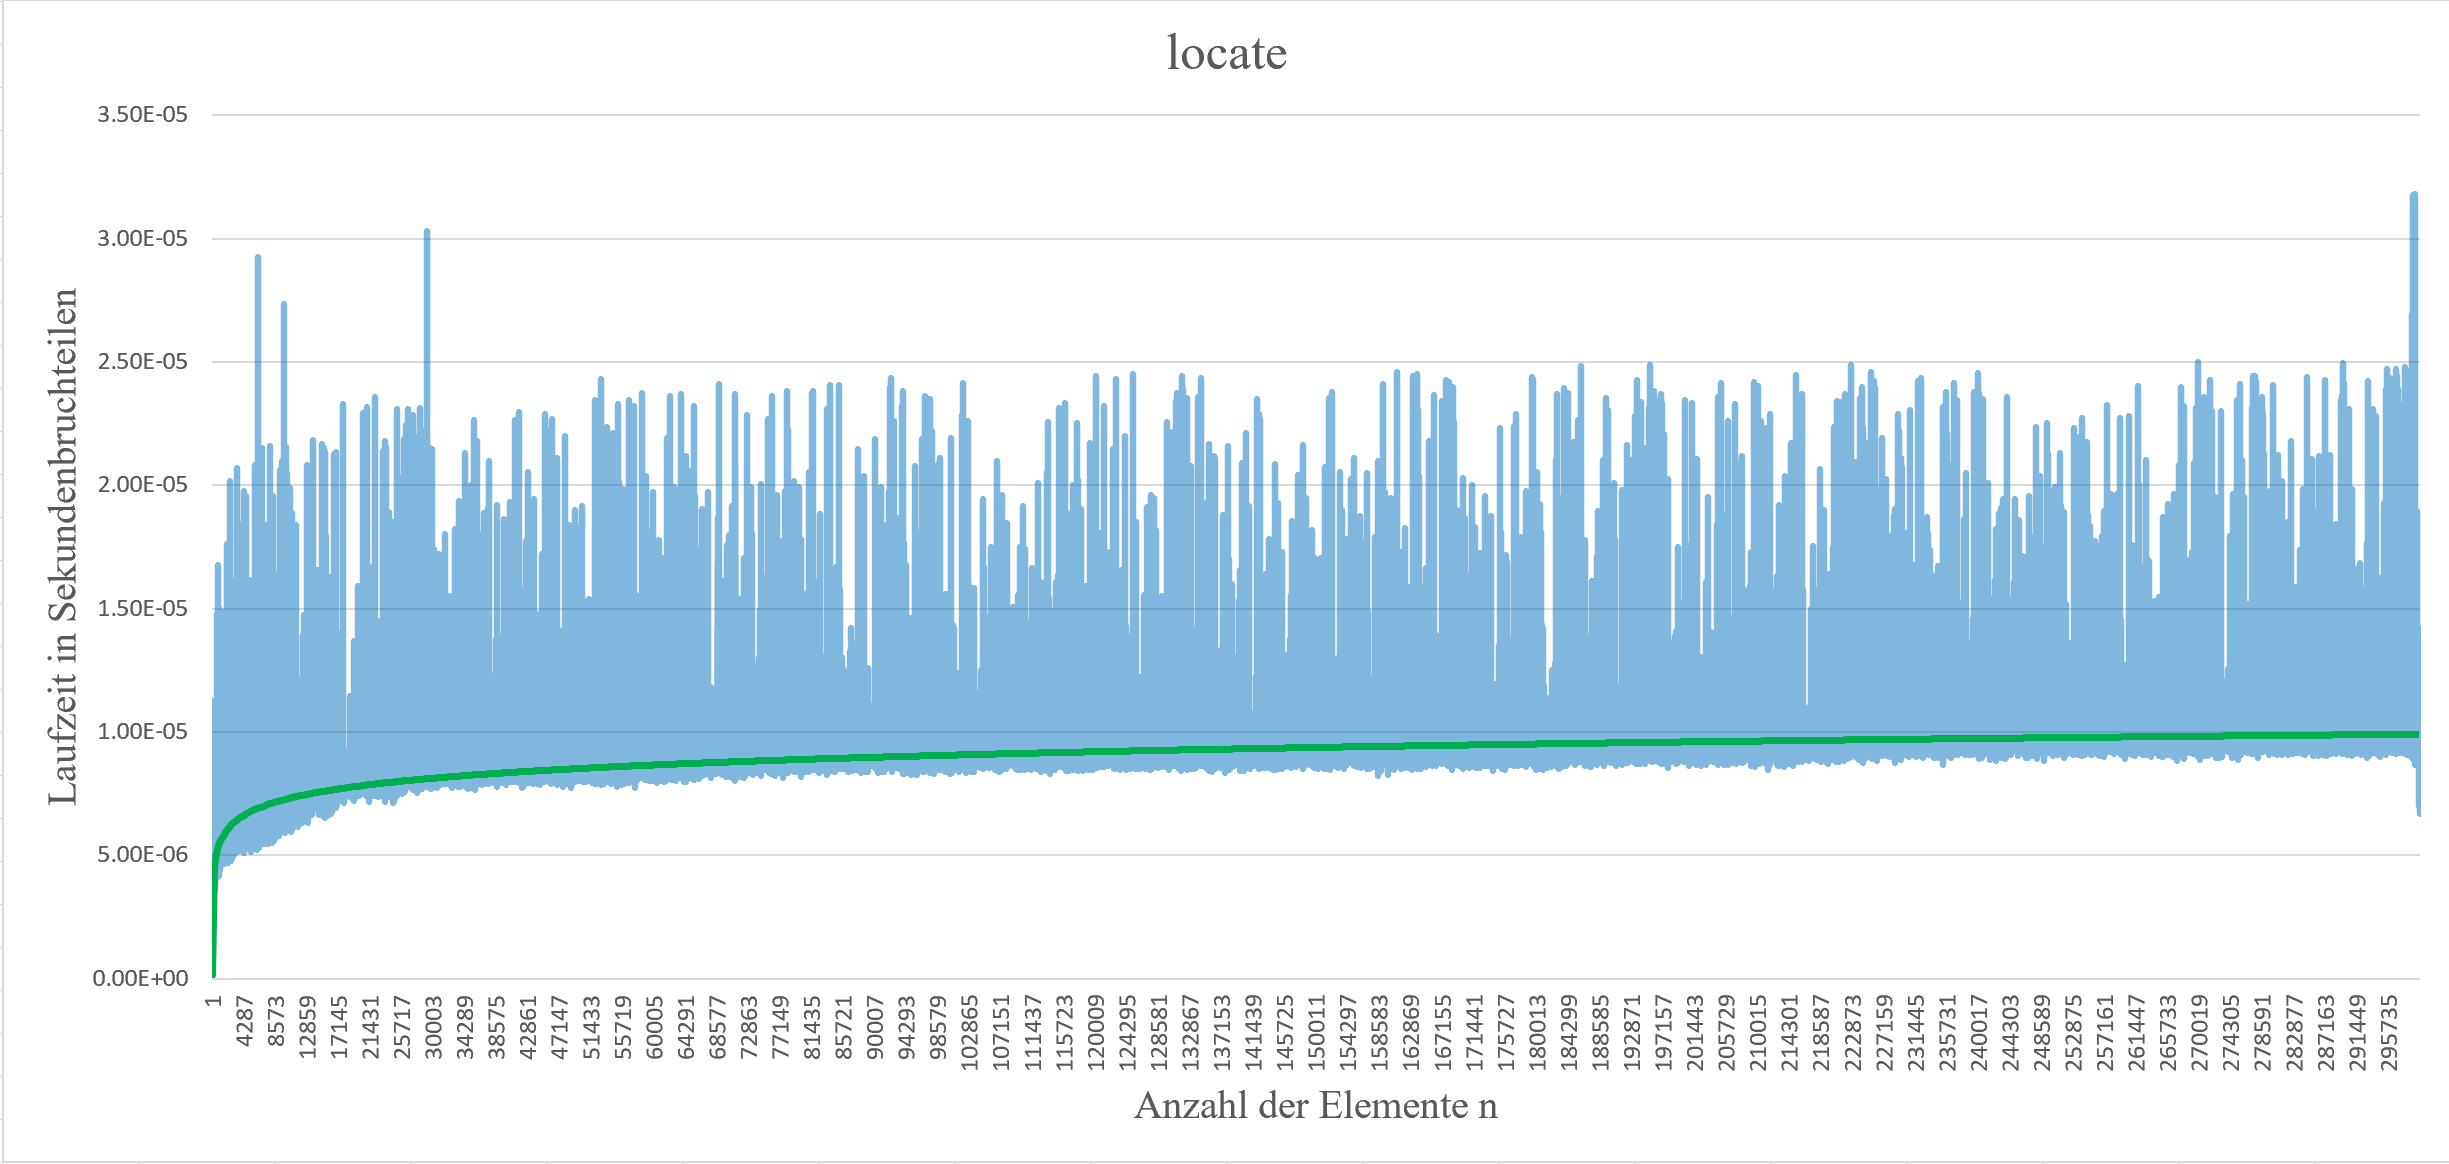
\includegraphics[width=\linewidth]{assets/benchmark300.png}
        \caption{Test von \texttt{locate} mit 0 bis 300.000 Elementen, blau dargestellt sind die Messwerte, grün die Trendlinie.}
        \label{fig:benchmark300}
    }
\end{figure}

\par
Die Daten von \autoref{fig:benchmark300} sind zwar schon beeindruckend, aber sagen ohne einen Vergleich noch relativ wenig aus. Deshalb führte ich den gleichen Test mit meiner Implementation der doppelt verketteten Liste durch. Der Vergleich der Trendlinien der beiden Testergebnisse ist in \autoref{fig:listvstree} zu sehen. Ich beschränkte mich hierbei auf ein Maximum von 250 Elementen, da schon so die unterschiedliche Entwicklung der Graphen auf eine beeindruckende Art und Weise zu erkennen ist.

\begin{figure}
    \centering{
        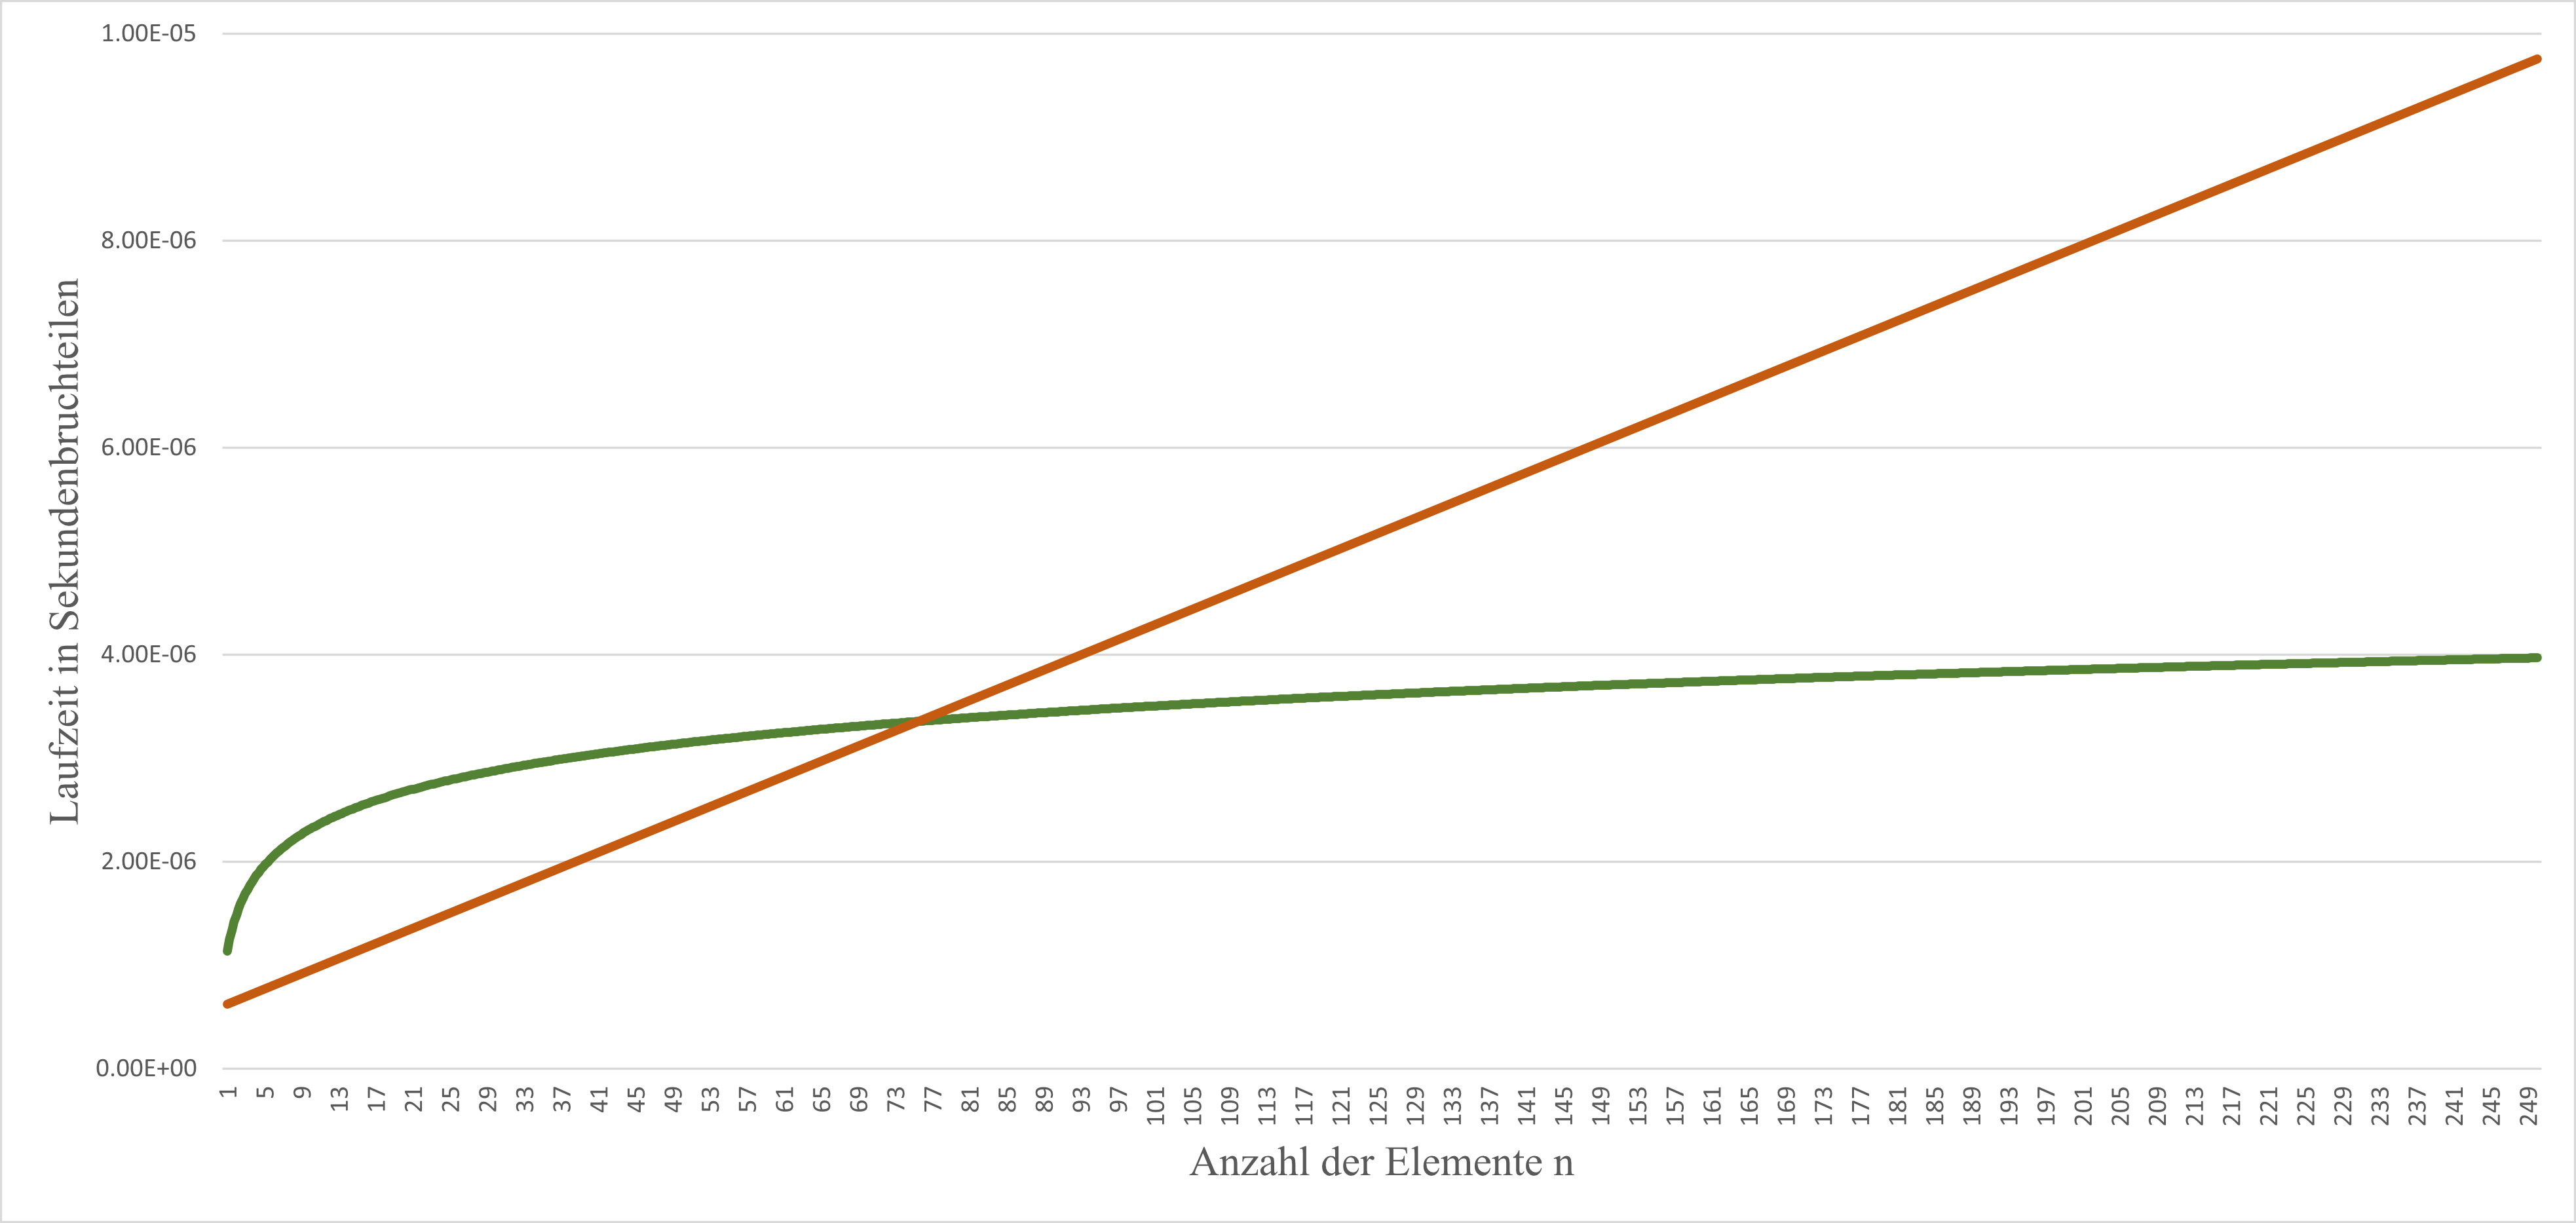
\includegraphics[width=\linewidth]{assets/listvstree.png}
        \caption{Die Trendlinien der Ergebnisse des Testes an (a,b)-Bäumen (grün) und doppelt verketteten Listen im Bereich von $0 < n \leq 500$ zeigen die Überlegenheit von (a,b)-Bäumen eindrucksvoll.}
        \label{fig:listvstree}
    }
\end{figure}
